\documentclass[../main.tex]{subfiles}

\begin{document}

\chapter{Introduction}\label{cha:introduction}
\todo{Things to say here:
  \begin{itemize}
    \item \cps{} are systems in which computers and physical machines are tightly coupled.
    \item Increase of large-scale problems Nowadays problems (some examples)
    \item Security problems in those systems \\Here I can give some examples such as Stuxnet \cite{Langner2011}, Brazil blackouts in 2010 \cite{Conti2010}, Ukraine Power System Attack and other attacks (use examples in~\cite{DingEtAl2018,Bindra2017})%
  \end{itemize}
  maybe use https://csiac.org/articles/security-of-cyber-physical-systems/??
}
[[id:~/docsThese/bibliography/DibajiEtAl2019.pdf-annot-3-13][Examples of CPS cyber-attacks]]
\cite{DibajiEtAl2019}

A more bibliometric approach with trends in control can be seen in~\cite{ZacchiaEtAl2019}.

\section{Motivation and Contributions}
Due to the increased computation capabilities of computers in recent years, now we can solve some problems that were not solvable in a reasonable time.
Thus the \emph{renaissance} of some optimization based methods, such as \todo{Neural networks} and \todo{Artificial Intelligence}.
For other more common methods such \mpc~\cite{GarciaEtAl1989}, this development meant solving more significant problems in less time, sometimes even in realtime~\todo[add realtime MPC]{\cite{BesselmannEtAl2008}} and using small computation units that can fit in the palm of a hand~\cite{BanguraMahony2014}.
Nevertheless, the calculation is still expensive for some large-scale systems, and we need subterfuges, such as distributing it into different computation units.
As we will see, one of these strategies is called \dmpc.

This work studies what happens when these computation units do not work collaboratively.
Moreover, for a specific \dmpc{} framework, we search for a method to mitigate the effects of this non-cooperative behavior.

To give a general view to the reader and to serve as a main take-away of the possible effects of non-cooperative behaviors, we give a simple qualitatively example, which will be retaken in another section of this work, giving more insight into its causes.

\begin{example}[Effects of a malicious agent]\label{ex:qualitative_example}
  \todo{Maybe I can give directly the district heating example as shown in the poster for NecSys. Add an image to represent the district?\\}
  Imagine we have a large system whose overall objective (cost, comfort etc) we want to optimize, but its sub-parts are coupled.
  To solve this problem, a number of \emph{agents interact}.

  In the decomposition used in this work the agents need to exchange values with another agent which referees what we call a \emph{negotiation}. This referee we call \emph{coordinator}.
  The coordinator sends all agents a message, personalized for each agent, which we will call $\theta_{i}$. The indices $i$ indicate the number of the agent.
  In return, each agent responds the coordinator by sending a message, which we will call $\lambda_{i}$.
  This message $\lambda_{i}$ usually depends on the message $\theta_{i}$.\\
  We can see a scheme of the exchanges in Fig.~\ref{fig:ex_exchange_agents}

  % \pagebreak

  % \begin{minipage}[t]{1.0\linewidth}
  %   \vspace{.25cm}
  % \end{minipage}
  \begin{figure}[H]
    \centering
    \begin{tikzpicture}[font=\small,thick,node distance=3*0.6180cm and 0.6180cm,every node/.style=rectangle,
      mpcSmall/.style={fill=mpc_agent, minimum height=0.6180*2cm, minimum width=2cm},
      coordinator/.style={fill=mpc_coordinator, minimum height=0.6180*3cm, minimum width=6cm},
      ]

      \node[draw, mpcSmall,] (block1) {\small Agent 1};
      \node[fill=none, draw=none, right=of block1,] (mult) {\bf $\dots$};
      \node[draw, mpcSmall, fill=mpc_agent, right=of mult,] (blockM) {\small Agent M};
      \node[draw, coordinator, below=of mult,] (coordinator) {Coordinator};

      \draw[-latex,line width=1pt,red] (block1.south)+(0.4,.0) -- ( coordinator.north -| {$(block1.south)+(0.4,.0)$}) node [right,midway] {$\lambda_{1}$\ \faUserSecret};
      \draw[latex-,line width=1pt] (block1.south)+(-0.4,0) -- (  coordinator.north -| {$(block1.south)+(-0.4,0)$}) node [left,midway] {$\theta_{1}$};
      \draw[-latex,line width=1pt] (blockM.south)+(0.4,.0) -- ( coordinator.north -| {$(blockM.south)+(0.4,.0)$}) node [right,midway] {$\lambda_{M}$};
      \draw[latex-,line width=1pt] (blockM.south)+(-0.4,0) -- (  coordinator.north -| {$(blockM.south)+(-0.4,0)$}) node [left,midway] {$\theta_{M}$};
    \end{tikzpicture}
    \caption{Exchange between agents and coordinator.}\label{fig:ex_exchange_agents}
  \end{figure}
  Observe in Fig.~\ref{fig:ex_exchange_agents} that agent 1 sends a suspicious $\lambda_{1}$. Instead of sending the message it was supposed to send, it modifies it before sending to the coordinator.
  This can be considered as a \fdi{} attack, as we will see later (\S~\ref{sec:anomalous}).

In this example we have a system with $4$ agents and a coordinator. The objective is to minimize a given function $J$. While all other agents work cooperatively, agent 1 is ill-intentioned. In Fig.~\ref{fig:change_in_j}, we can see the effects of changes in the $\lambda_{1}$ sent on the objectives of each agent $J_{i}$ and the overall objective $J^{\star}$ (in blue).
  \begin{figure}[H]
    \centering
    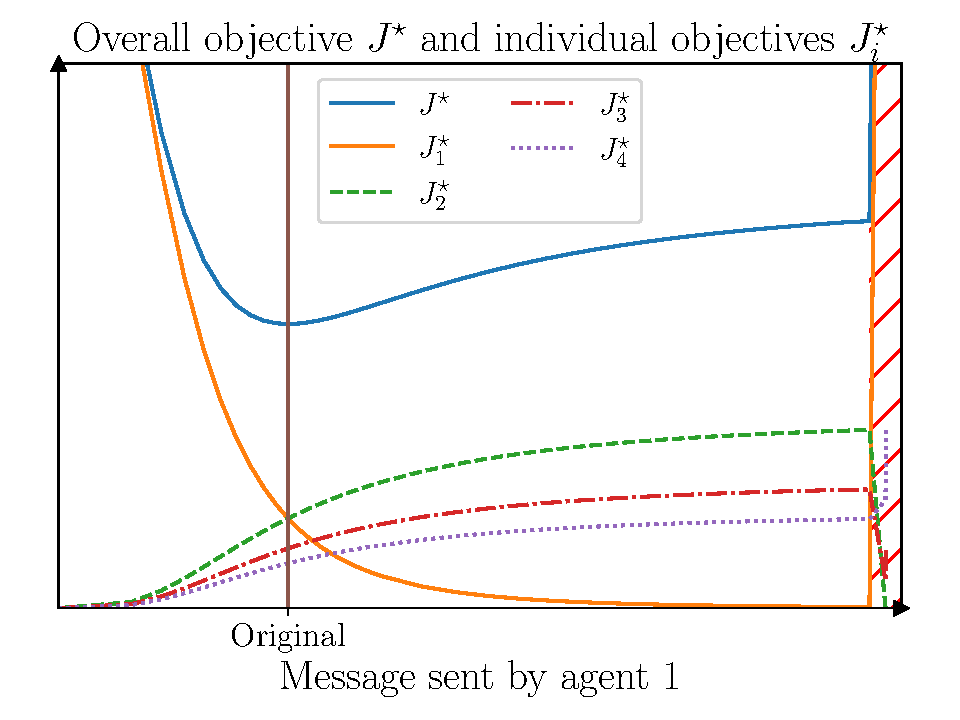
\includegraphics[width=.5\textwidth]{../img/qualitative_example.pdf}
% ./docstheseplot -o ../../docs/img/quantiteAvecTriche4 -i  ../../data/matlab/tricheQuantite/dmpcQuantity4systemsTriche_.mat --quantiteAvecTriche4
    \caption{Changes in objectives depending on message sent by agent 1.}\label{fig:change_in_j}
  \end{figure}
  Observe that the blue curve has its minimum value only when the $\lambda_{1}$ is the original one, every other message makes the resulting system sub-optimal.

  On the other hand we can see that agent 1 can manipulate the negotiation so it can privileged itself (orange curve) at the expense of all others (green, red and purpler curves). This selfish behavior can even destabilize the system, represented by the red hatched area on the graph.
\end{example}

From example~\ref{ex:qualitative_example}, we can see the two main effects of a attack: Loss of optimality and eventually \todo{total breakdown} of the system.

While one of them can sometimes be acceptable (depending on the suboptimality), the other is absolutely inadmissible, principally when we are talking about \cps{} that are essential, like electricity and water supply for instance.

So, our goal is to reduce those effects as much as possible.
And to guide us on the quest to minimize them, we can raise some questions:

\simplebox{
  \begin{itemize} \bfseries
    \item Can we detect an attack?
    \item Can we identify the ill-intentioned agent(s)?
    \item Can we mitigate the effects of the attack?
  \end{itemize}
}
This work has as objective to answer these questions, at least for specific cases which will be formally presented.

To understand and answer those questions, we divide this work into two parts.

\paragraph{Part~\ref{part:mpc_intro}} It serves as a gentle introduction to \dmpc{} and attacks.

For a unfamiliar reader, Chapter~\ref{sec:decomposing_mpc} explains what is a \mpc{} to begin with and shows some of the challenges to decompose it.
Chapter~\ref{sec:topoly_trust} discuss possible topologies used for those decompositions.
In Chapter~\ref{sec:anomalous} we define anomalous behaviors (and more specifically attacks), we categorize them and present some methods used in the literature to prevent and combat them.

\paragraph{Part~\ref{part:safe_dmpc}} It contains the contributions of this work.

Chapter~\ref{sec:primal_decomposition} presents the decomposition studied in this work (primal decomposition), some of its vulnerabilities and how they can affect the performance of the system (here we take up Example~\ref{ex:qualitative_example} giving it a more quantitative approach).
Once we know the vulnerabilities and possible effects of attacks, we divide the mitigation problem into manageable parts.
\\ First in Chapter~\ref{sec:safe_pddmpc_eq}, we analyze an unsophisticated problem, so we can assess the difficulties that can be found when solving the mitigation problem. From the analysis of the problem we propose a detection and mitigation mechanism, followed by an academical example to illustrate.
\\Then, in Chapter~\ref{sec:safe_pddmpc_ineq}, we analyze a similar problem but with a twist. As we will see, just one small modification on the initial problem can increase exponentially its complexity.
From the analysis of the newly-found problem we propose a similar strategy, but with adequate modifications to contain the exponential nature of the problem.
\todo{\\Finally, we continue in Chapter~\ref{sec:safe_pddmpc_ineq_reconst} the methodology and explore some more properties to create a less conservative strategy.}
\todo{\\Maybe if the time permits modify the cheating device??}
\\Then, we conclude this work in Chapter~\ref{sec:conclusion} with a discussion about the results found during this study, benefits as well as shortcomings. Some of this discussion leads to open questions which can incite new works.

% Since those questions are still open, this work has as objective to discuss these questions by analyzing the recent literature and schematizing the security in decomposition methods for Model Predictive Control passing by the following items:
% \begin{itemize}[label=$\bullet$]
%   \item decomposition methods;
%   \item topology;
%   \item points of vulnerability;
%   \item how malicious agents can benefit from such vulnerabilities;
%   \item effects on the overall system;
%   \item possible ways to mitigate.
% \end{itemize}
% We use some conclusions of the discussion to develop safe algorithms for a \dmpc\ framework.

\section{Publications}
The work and discussion presented in this thesis yielded the following publications
\begin{itemize}
  \item Published
        \begin{description}
          \item[\cite{NogueiraEtAl2021}] Conference article for the SysTol'21
          \item[\cite{NogueiraEtAl2022}] \todo[correct citation]{} Conference article for the NecSys'22
        \end{description}
  \item Under Review
  \item In Preparation
\end{itemize}



% \chapterEndOrnament

\end{document}
